\chapter{Introduction}

LoRaWAN uses the proprietary chirp spread spectrum radio modulation
LoRa to achieve long range (\textgreater{}10~km) connectivity, while
maintaining low energy consumption. The protocol definition and related materials are published by the LoRa Alliance \cite{spec}.
As LoRaWAN is designed for internet of things (IoT)
devices, it provides very low bandwidth (between 292~bit/s and 50~kilobit/s) at very low energy consumption (100~nA -- 10~mA) \cite{wiki_de_lorawan}. Devices are
usually built using a microcontroller only and do not contain a
full-fledged operating system.

A summary of the LoRaWAN standard \cite{spec} follows.

LoRaWAN devices can operate in two different modes:

\begin{itemize}
\tightlist
\item
  {ABP (activation by personalisation)}
\item
  {OTAA (over the air activation)}
\end{itemize}

{The first mode, ABP, requires configuring two symmetric keys and a
device address per device:}

\begin{itemize}
\tightlist
\item
  {AppSKey}
\item
  {NwkSKey}
\item
  {DevAddr}
\end{itemize}

{With ABP, devices are pre-configured and never change keys nor need any
join procedure.}


{With OTAA, devices are configured with}

\begin{itemize}
\tightlist
\item
  {AppEUI}
\item
  {AppKey}
\end{itemize}

{Devices using OTAA use a join procedure for joining the network: First
the devices sends a Join-Request message to the network, which replies
with a Join-Accept message. AppSKey and NwkSKey are computed in this
procedure.}

{The two message in the standard are defined as follows:}

\begin{figure}[h!]
{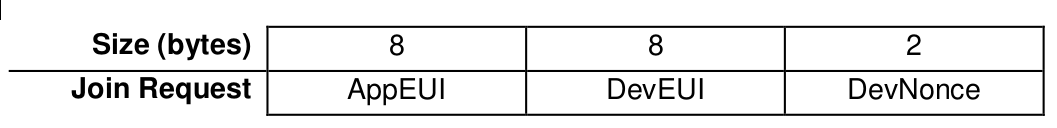
\includegraphics[width=0.8\textwidth]{images/image16.png}}
\end{figure}

\begin{figure}[h!]
{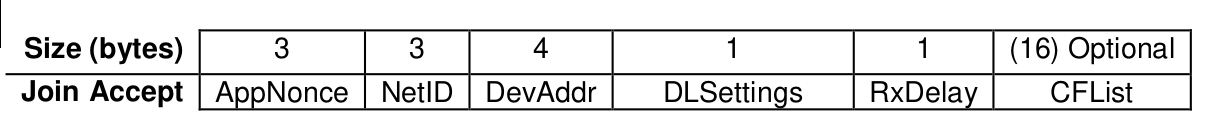
\includegraphics[width=0.8\textwidth]{images/image6.png}}
\end{figure}

{(both images copied from the LoRaWAN standard)}


{When using OTAA, the AppSKey and NwkSKey are determined as follows:}

\begin{figure}[h!]
{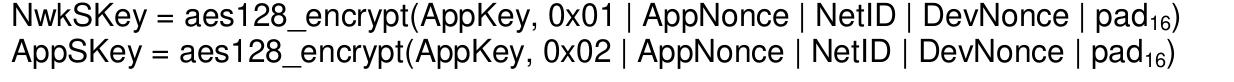
\includegraphics[width=0.8\textwidth]{images/image4.png}}
\end{figure}

{(also copied from the standard)}

{Note that both the AppSKey and the NwkSKey are derived from the AppKey.
We will elaborate on this aspect later.}

\section{Security mechanisms in LoRaWan}

{The standard defines the following security mechanisms:}

\subsection{Payload encryption}

{The payload of the message is encrypted using AES with 128-bit keys.
The contents of the payload is thereby hidden from the attacker (except
for its length). However, several important fields are
not considered payload and therefore are sent in cleartext, namely:}

\begin{itemize}
\tightlist
\item
  {DevAddr: the device address -- a device identifier. This identifies
  the device permanently in case of ABP or per-session in case of OTAA.
  A session can be arbitrarily long-lived, as re-initialization is not
  specified by the standard.}
\item
  {FCnt: the frame counter. For both uplink and downlink messages, this
  is incremented each time a message from/to this device is sent (modulo
  $2^{16}$).}
\item
  {FCtrl and FOpts: contain settings for the frame and transmission. May
  identify the device type or manufacturer, as they depend on the
  capabilities of the device.}
\item
  {FPort: a field used for multiplexing inside the application. This is
  application-level information, so it may be sensitive, but it is sent
  outside of the payload. The authors are surprised by this decision.}
\end{itemize}

\subsection{Message integrity protection}

{The important parts of the message (in particular all of the above
fields) are protected by a Message Integrity Code derived from an
AES-based MAC. The MAC is keyed by NwkSKey in case of messages to the
network or AppSKey for application messages. The frame counter is part
of the MAC calculation to prevent MIC re-use.}

\subsection{Replay attack protection}

{The standard defines that the frame counter may only increase in order
to prevent replay attacks. Any packets with a frame counter lower than
the last seen value should be discarded. However, in practice it is hard
to implement a device that behaves accordingly: a LoRa device may lose
power anytime, and storing the frame counter in non-volatile storage
after every message is often seen as
infeasible.\footnote{LoRa devices are usually power-constrained and writing data to non-volatile storage costs extra energy. Perhaps more importantly, it limits the lifetime of the device, because flash storage can only sustain a limited number of overwrites (on the order of thousands for a single cell).} Therefore
all providers in Switzerland give the option to ignore the frame
counter: in this mode, a packet with a frame counter of 0 is allowed any
time, with the extra effect of dropping any further packets with high
counters.}

\chapter{General Security issues}

\section{Incomplete Standard}

{While the LoRaWAN standard defines several entities, it does not define
the network provider entity clearly. Specifically, it does not define
how key distribution happens, who defines the symmetric keys used or how
they are exchanged. As LoRaWAN security is based on symmetric keys, the
lack of a definition poses security risks in leakage of keys during
configuration/distribution of devices.}

\section{Key Management}

{When using OTAA, the NwkSKey and AppSKey are calculated by the network.
In theory the network provider could contact a service of the owner of
the IoT device to retrieve the NwkSKey and thus not have access to the
AppSKey nor the AppKey. In practice, this does not happen: in all
network providers that we checked in Switzerland (Swisscom, TTN,
Loriot), the network provider itself calculates both keys.}

{Even though the separated setup has been discussed in the TTN
community, there is no implementation available that supports this
separation.}

{The two different AES keys that are defined by the standard, can
practically be seen as only one key, as they are derived from the same
master key. Thus the objective to protect data from the network provider
with two different keys is not achieved in reality. The network provider
can decrypt and manipulate all messages, unless additional
application-layer security is introduced.}

\section{\texorpdfstring{{Static
keys}}{Static keys}}\label{h.1g22hul9yfrw}

{When using ABP, the session keys are fixed and will never be replaced.
Thus brute force attacks can use every packet the device sends during
its whole lifetime, and leaked keys compromise all future packets until
manual re-configuration.}

\section{\texorpdfstring{{Preconfigured
devices}}{Preconfigured devices}}\label{h.7mkfizapvt5a}

{The test devices that were ordered from Ascoel
(\href{http://www.ascoel.it}{www.ascoel.it})
contained pre-configured keys. While this might be convenient in some
places, it also allows the manufacturer to decrypt the data sent by the
devices. Furthermore the devices came pre-configured in ABP mode and
thus never change the session keys. For some devices it was impossible
to change the keys or switch to OTAA mode.}

\section{\texorpdfstring{{Replay
attacks}}{Replay attacks}}\label{h.eymg8atzq5bp}


{The LoRaWAN standard defines counters in the frame header:}

\begin{figure}[h!]
{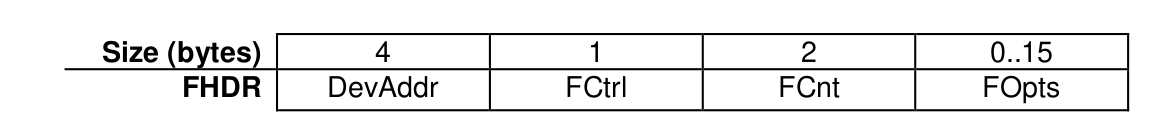
\includegraphics[width=0.8\textwidth]{images/image9.png}}
\end{figure}

{While in theory they should always be increasing during one session, in
practice all network providers offer at least to ignore the counter. ABP
devices always use the same session and thus when the battery is
replaced, the counter will be reset (as usually this is not stored in
non-volatile memory). Thus network providers allow frame counter reset.}

{Thus an attacker has the ability to replay packets for ABP devices, if
the network provider is configured to ignore the frame counter.}

{In OTAA the session is restarted every time the device follows the join
procedure and thus it uses fresh session keys. It is though undefined,
how often or if at all the device repeats the join procedure. The join
request itself does not have any protection against replay attacks.}

\hypertarget{h.1a3modh2fhpw}{\chapter{\texorpdfstring{{Security of
event-based
devices}}{Security of event-based devices}}\label{h.1a3modh2fhpw}}

\hypertarget{h.kyg6ihxrou88}{\section{\texorpdfstring{{Motivation}}{Motivation}}\label{h.kyg6ihxrou88}}

{While it was show in the previous section that there are various
obvious security issues within LoRaWAN, the nature of a long range
wireless network allows attacks from a far away adversary that are not
possible with traditional wireless protocols like 802.11. If a device
sends a message, it can be detected within the range of a receiver,
which might be within a couple of kilometers distance.}

\section{Use cases and
List of devices}\label{h.jsdk7si1wtbx}

{To illustrate the potential threats, a list of event based devices
found on the market has been compiled. The attack vectors assume that
the devices only send a message if an event has happened.}

\begin{longtable}[c]{|l|l|l|}
\hline
\begin{minipage}[t]{0.20\columnwidth}\raggedright\strut
\textbf{Category}
\strut\end{minipage} &
\begin{minipage}[t]{0.30\columnwidth}\raggedright\strut
\textbf{Use case(s)}
\strut\end{minipage} &
\begin{minipage}[t]{0.40\columnwidth}\raggedright\strut
\textbf{Attack vector / examples}
\strut\end{minipage}\tabularnewline
\hline
\begin{minipage}[t]{0.20\columnwidth}\raggedright\strut
{Water sensors}
\strut\end{minipage} &
\begin{minipage}[t]{0.30\columnwidth}\raggedright\strut
{Detect overflowing bath tub, broken pipe}
\strut\end{minipage} &
\begin{minipage}[t]{0.40\columnwidth}\raggedright\strut
\begin{itemize}
\tightlist
\item
  {A fake plumber could approach the house and get access, as the person
  knows that there is a water leakage.}
\item
  {Replay attacks could be used to cause a real plumber to visit the
  house and cause unnecessary costs}
\end{itemize}
\strut\end{minipage}\tabularnewline
\hline
\begin{minipage}[t]{0.20\columnwidth}\raggedright\strut
{Burglar alarm}
\strut\end{minipage} &
\begin{minipage}[t]{0.30\columnwidth}\raggedright\strut
{Detects if somebody is in the house, sends alarm if movement is
detected.}
\strut\end{minipage} &
\begin{minipage}[t]{0.40\columnwidth}\raggedright\strut
\begin{itemize}
\tightlist
\item
  {As above}
\end{itemize}
\strut\end{minipage}\tabularnewline
\hline
\begin{minipage}[t]{0.20\columnwidth}\raggedright\strut
{Smoke detector}
\strut\end{minipage} &
\begin{minipage}[t]{0.30\columnwidth}\raggedright\strut
{Detect smoke/fire in a house}
\strut\end{minipage} &
\begin{minipage}[t]{0.40\columnwidth}\raggedright\strut
\begin{itemize}
\tightlist
\item
  {As above}
\end{itemize}
\strut\end{minipage}\tabularnewline
\hline
\begin{minipage}[t]{0.20\columnwidth}\raggedright\strut
{Radioactivity detector}
\strut\end{minipage} &
\begin{minipage}[t]{0.30\columnwidth}\raggedright\strut
{Detect radiation}
\strut\end{minipage} &
\begin{minipage}[t]{0.40\columnwidth}\raggedright\strut
\begin{itemize}
\tightlist
\item
  {Cause panic using replay attacks}
\end{itemize}
\strut\end{minipage}\tabularnewline
\hline
\begin{minipage}[t]{0.20\columnwidth}\raggedright\strut
{Buttons}
\strut\end{minipage} &
\begin{minipage}[t]{0.30\columnwidth}\raggedright\strut
{Sends an event when pressed. Can be used as emergency notification
(``HELP'') or in case something is broken (``Repair requests'')}
\strut\end{minipage} &
\begin{minipage}[t]{0.40\columnwidth}\raggedright\strut
\begin{itemize}
\tightlist
\item
  {Similar to water sensors}
\end{itemize}
\strut\end{minipage}\tabularnewline
\hline
\begin{minipage}[t]{0.20\columnwidth}\raggedright\strut
{Remote controls}
\strut\end{minipage} &
\begin{minipage}[t]{0.30\columnwidth}\raggedright\strut
{Control light, power, TV, windows with a LoRaWAN based remote control}
\strut\end{minipage} &
\begin{minipage}[t]{0.40\columnwidth}\raggedright\strut
\begin{itemize}
\tightlist
\item
  {Adversary can learn about the presence of people in the house}
\item
  {Susceptible to replay attacks}
\end{itemize}
\strut\end{minipage}\tabularnewline
\hline
\begin{minipage}[t]{0.20\columnwidth}\raggedright\strut
{Parking sensor}
\strut\end{minipage} &
\begin{minipage}[t]{0.30\columnwidth}\raggedright\strut
{Detects if a parking lot is used or free.}
\strut\end{minipage} &
\begin{minipage}[t]{0.40\columnwidth}\raggedright\strut
\begin{itemize}
\tightlist
\item
  {Adversary can learn about occupation of parking house and possibly
  can infer business success from the usage.}
\end{itemize}
\strut\end{minipage}\tabularnewline
\hline
\begin{minipage}[t]{0.20\columnwidth}\raggedright\strut
{Bluetooth sensor}
\strut\end{minipage} &
\begin{minipage}[t]{0.30\columnwidth}\raggedright\strut
{If a paired device (usually a smart phone) is out of range, an alarm is
being sent.}
\strut\end{minipage} &
\begin{minipage}[t]{0.40\columnwidth}\raggedright\strut
\begin{itemize}
\tightlist
\item
  {Adversary can learn that the object or the phone is lost (and look
  for it, too)}
\end{itemize}
\strut\end{minipage}\tabularnewline
\hline
\begin{minipage}[t]{0.20\columnwidth}\raggedright\strut
{Animal tracking}
\strut\end{minipage} &
\begin{minipage}[t]{0.30\columnwidth}\raggedright\strut
{The position of an animal is sent when motion is detected.}
\strut\end{minipage} &
\begin{minipage}[t]{0.40\columnwidth}\raggedright\strut
\begin{itemize}
\tightlist
\item
  {Adversary can learn about the behaviour of animals, infer information
  at a distance}
\end{itemize}
\strut\end{minipage}\tabularnewline
\hline
\end{longtable}

{While LoRaWAN uses AES encryption, it can be seen from the above list
that sending (or not sending) a message might be enough information for
an adversary to infer significant knowledge about the objects in
question.}
\section{\texorpdfstring{{Example: Door
sensor}}{Example: Door sensor}}\label{h.bju94okea6h3}

The Ascoel CM868 door
sensor\footnote{\url{http://www.ascoel.it/images/pdf_ascoel/CM868LRTH_eng.pdf}} was shipped
to us with pre-defined ABP keys and DevAddr. To be usable in TTN or any
other Swiss network provider, the DevAddr and keys need to be changed.
However, according to the manufacturer, the current firmware does not
support changing the address nor keys. Thus the device was not usable in Switzerland.

Even if the device were
usable, any user of this device would share the key with the
manufacturer and could never change the key herself. No further tests
have been conducted with this device, as debugging without access to the
packets (as hardcoded keys were used) and thus the data was not seen
feasible.

\section{\texorpdfstring{{Example:
Burglar alarm}}{Example: Burglar alarm}}\label{h.ajy5u48pfd5q}

{The Ascoel IR868LR family\footnote{\url{http://www.ascoel.it/images/pdf_ascoel/IR868LR_eng.pdf}} is
an infrared passive sensor for indoor applications. It is also shipped
in ABP mode with pre-configured keys. It can, however, be reconfigured
to OTAA and the parameters can be changed (DevAddr, NwSKey, AppSKey for
ABP and AppEUI and AppKey for OTAA). After changing the device to OTAA,
packets are being sent to the network:}
\begin{enumerate}
\tightlist
\item
  {special packets after the device started}
\item
  {keep-alive packets every couple of minutes}
\item
  {an alarm packet when presence is detected}
\end{enumerate}
{While all of these messages can be distinguished when the keys are
known, the type of these messages can also be understood by an
adversary, without the key knowledge, because the device uses different
ports for different types of messages and the port is being sent in
plaintext as specified by the LoRaWAN standard:}
\begin{figure}[h!]
{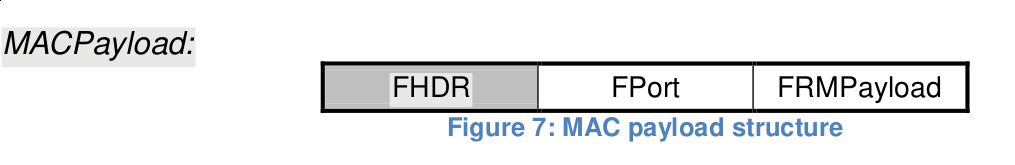
\includegraphics[width=0.8\textwidth]{images/image13.png}}
\end{figure}
{The following graph, depicting the ports of packets in time, was
created from the received packets of the device:}
\begin{figure}[h!]
{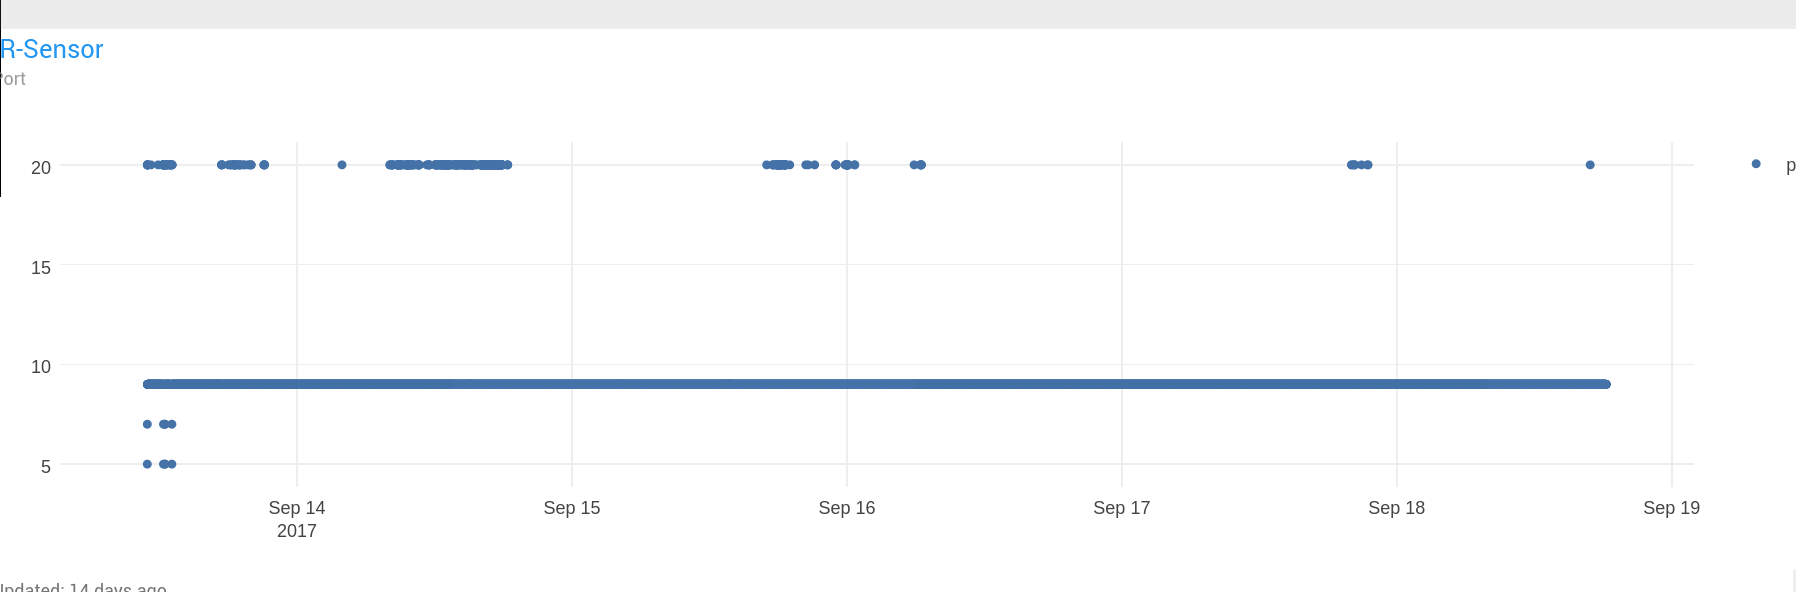
\includegraphics[width=0.8\textwidth]{images/image3.png}}
\end{figure}

{It can be seen that the keep-alive packets are being sent on port 9,
boot-up messages on port 5, and the presence detection uses port 20.
While these packets were received using the correct keys, the port
information is known to any adversary in range of the device.}

\section{\texorpdfstring{{Counter-measurements}}{Counter measurements}}\label{h.5p1f7221qm42}

{If event-based devices are not time critical (such as e.g. parking
sensors), they can opt for sending packets in fixed time intervals to
hide the events.}

{We assume that the motivation of the manufacturer to use different
ports was to make life easier for developers. However, as it is sent in
plain text, information is revealed unencrypted to an adversary. This
problem could easily be fixed, by including the message type within the
encrypted payload and always using the same port. This would have to be
done on the application level, as encryption of the port itself is not
possible in the current standard.}

\hypertarget{h.6snn4dp8j73u}{\section{\texorpdfstring{{LoRaWAN Standard
and changes in LoRaWAN
1.1}}{LoRaWAN Standard and changes in LoRaWAN 1.1}}\label{h.6snn4dp8j73u}}

{One of the biggest changes in LoRaWAN 1.1 is the addition of the
backend definition. Details of this will be discussed below.}

\hypertarget{h.jpbc1i7c9eqd}{\subsection{\texorpdfstring{{Frame
counters}}{Frame counters}}\label{h.jpbc1i7c9eqd}}

{The LoRaWAN 1.1 standard defines 3 instead of 2 frame counters. While
1.0 defined one frame counter for uplink messages, 1.1 defines one
counter for messages with fport = 0 and one counter for all other uplink
counters. All frame counters are now 32 bit values. More importantly
}{LoRaWAN 1.1 forbids frame counter resets}{. Specifically it says}

{``ABP devices have their Frame Counters initialized to 0 at
fabrication. In ABP devices the}

{frame counters MUST NEVER be reset during the device's life time. If
the end-device is}

{susceptible of losing power during its life time (battery replacement
for example), the frame}

{counters SHALL persist during such event.''}

{And}

{``The end-device shall not reuse the same FCntUp value, except for
retransmission, with the}

{same application and network session keys.''}

{In case of OTAA/Network join, the counter is called devnonce and is
resetted on every join:}

\begin{figure}[h!]
{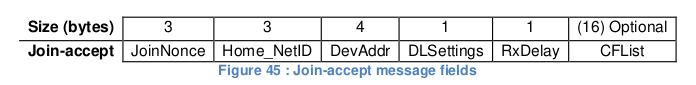
\includegraphics[width=0.8\textwidth]{images/image14.png}}
\end{figure}

{``DevNonce is a counter starting at 0 when the device is initially
powered up and incremented}

{with every Join-request. A DevNonce value SHALL NEVER be reused for a
given JoinEUI}

{value. If the end-device can be power-cycled then DevNonce SHALL be
persistent (stored}

{in a non-volatile memory). Resetting DevNonce without changing JoinEUI
will cause the}

{Network Server to discard the Join-requests of the device. For each
end-device, the}

{Network Server keeps track of the last DevNonce value used by the
end-device, and}

{ignores Join-requests if DevNonce is not incremented.``}

{Thus ABP devices need to have a permanent storage for their frame
counter, while OTAA devices can keep their counter in volatile memory,
because they can reset their counter with new keys with a new join
request.}

{However OTAA devices receive a JoinNonce from the network that will
always increase and thus needs to be stored in non-volatile memory:}

{``Note: This mechanism prevents replay attacks by sending previously
recorded join-request messages with the intention of disconnecting the
respective end-device from the network. Any time the Network Server
processes a Join-Request and generates a Join-accept frame, it shall}

{maintain both the old security context (keys and counters, if any) and
the new one until it receives the first successful uplink frame
containing the RekeyInd command using the new context, after which the
old context can be safely removed``}

\begin{figure}[h!]
{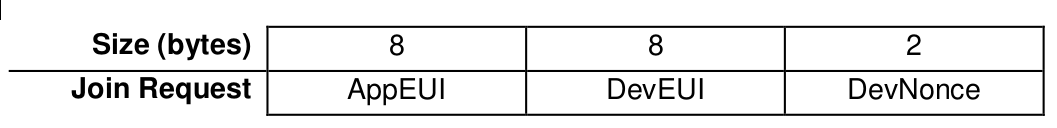
\includegraphics[width=0.8\textwidth]{images/image16.png}}
\end{figure}

{``The JoinNonce is a device specific counter value (that never repeats
itself) provided by the}

{Join Server and used by the end-device to derive the session keys
FNwkSIntKey, SNwkSIntKey, NwkSEncKey and AppSKey. JoinNonce is
incremented with every Join-}

{accept message.''}

{``The device keeps track of the JoinNonce value used in the last
successfully processed Join-}

{accept (corresponding to the last successful key derivation). The
device SHALL accept the}

{Join-accept only if the MIC field is correct and the JoinNonce is
strictly greater than the}

{recorded one. In that case the new JoinNonce value replaces the
previously stored one.}

{If the device is susceptible of being power cycled the JoinNonce SHALL
be persistent}

{(stored in a non-volatile memory).}

{The LoRa Alliance allocates a 24bits unique network identifier (NetID)
to all networks with}

{the exception of the following NetID values reserved for
experimental/private networks that}

{are left unmanaged.}

{``}

\hypertarget{h.6wjpqn9cabfu}{\subsection{\texorpdfstring{{The gap drop
is removed}}{The gap drop is removed}}\label{h.6wjpqn9cabfu}}

{While the 1.0 standard defined that when a counter with a too big gap
was detected, further frames are to be dropped, 1.1 removes this
definition. By the removal of it, denial of service attacks with replay
of packets are prevented.}

{``At the receiver side, the corresponding counter is kept in sync with
the}

{value received provided the value received has incremented compared to
the current}

{counter value and is less than the value specified by MAX\_FCNT\_GAP 1
after considering}

{counter rollovers. If this difference is greater than the value of
MAX\_FCNT\_GAP then too}

{many data frames have been lost then subsequent will be discarded.''}

\hypertarget{h.7ctbv6nd7du7}{\subsection{\texorpdfstring{{Channel
selection}}{Channel selection}}\label{h.7ctbv6nd7du7}}

{Both standards define that }

{``The end-device changes channel in a pseudo-random fashion for every
transmission. The resulting frequency diversity makes the system more
robust to interferences.''}

{In practise all tested devices just select the next channel for the
next packet. Thus an attacker can see if she did not receive a packet.
This might be particular useful for event based devices in which an
attacker wants to distinguish between regular noise and real events.}

\hypertarget{h.i6r97yb5iafg}{\subsection{\texorpdfstring{{FPort}}{FPort}}\label{h.i6r97yb5iafg}}

{The FPort is still unencrypted in LoraWAN 1.1. Thus the event
indications that were observed with the burglar alarm in our experiments
are still observable. To improve security, the LoRaWAN standard should
move the FPort part into the encrypted message part.}

\hypertarget{h.mdrkurwqvvj8}{\subsection{\texorpdfstring{{NEW: Lora
alliance DNS server as a single point of
failure}}{NEW: Lora alliance DNS server as a single point of failure}}\label{h.mdrkurwqvvj8}}

{The new standard defines to use the DNS names
}{JOINEUIS.LORA-ALLIANCE.ORG}{~and }{NETIDS.LORA-ALLIANCE.ORG }{that
SHALL be used for finding the join server and netid respectively.}

{In this regard the domain name }{LORA-ALLIANCE.ORG }{becomes a }{NEW
single point of failure }{for backend networks.}

{Compare with chapter ``19.1}{~DNS configuration'' of the backend
definition.}

\hypertarget{h.mn1ux3159m0}{\subsection{\texorpdfstring{{Communication
between gateway and the
network}}{Communication between gateway and the network}}\label{h.mn1ux3159m0}}

{In LoRaWAN 1.1 gateways are connected to the Network Server via secured
standard IP connections, while previously it was undefined. In practise
packets of LoRaWAN 1.0 gateways were forwarded using plain UDP without
any encryption or signature.}

\hypertarget{h.jom2i6adwnnm}{\subsection{\texorpdfstring{{NetID
defined}}{NetID defined}}\label{h.jom2i6adwnnm}}

{Before version 1.1 the handling of the NetID was undefined and could be
chosen by a network provider. Since 1.1 they are allocated by lora
alliance. Even though this will regulate the use more clearly, it also
adds an additional attack vector: Now an attacker can lookup the netid
from the DNS database and specifically attack a network}

\hypertarget{h.rext4wcd7qnn}{\subsection{\texorpdfstring{{Communication
between
AS/NS/JS}}{Communication between AS/NS/JS}}\label{h.rext4wcd7qnn}}

{The LoRaWAN 1.1 standard defines a reference backend network model as
follows:}
\begin{figure}[h!]
{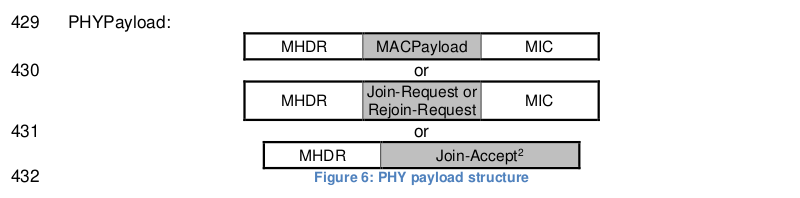
\includegraphics[width=0.8\textwidth]{images/image10.png}}
\end{figure}

{The LoRaWAN Standard defines only use of shared keys between the
application server / network server and join server. However public key
crypto would also be feasible (page 18 of backend document).}

\hypertarget{h.rxbla8bfpdr7}{\subsection{\texorpdfstring{{Unique Key
usage}}{Unique Key usage}}\label{h.rxbla8bfpdr7}}

{Version 1.1. defines that a key should be unique per device: }

{``1. Since all end-devices are equipped with unique application and
network root keys specific for each end-device, extracting the
AppKey/NwkKey from an end-device only compromises this one end-device.''
(6.1.1.3 footnote 1)}

{Prior to 1.1 this was undefined and thus shared keys were used in
different devices, especially for ABP devices.}

\hypertarget{h.ukt1jzew31xa}{\subsection{\texorpdfstring{{Key
Derivation}}{Key Derivation}}\label{h.ukt1jzew31xa}}

{One of the challenging aspects of LoRaWAN is a safe key derivation
method to separate payload and mac command encryption. LoRaWAN 1.0 does
not define the backend and thus left it open to the network provider on
which part of the infrastructure generates the keys. In practise this
led to the situation that network providers (TTN, Loriot, Swisscom) all
have knowledge of both keys and user data is visible to the network
provider.}

{Even though in LoRaWAN backend services are defined and the Join Server
handles the key management, it is highly unlikely that a user actually
operates the join server, as it takes a core role in the network
providers backend. }

{It is defined that the application server will request the keys from
the join server on arrival of encrypted messages with payload inside.
That means that the join server and the application server would need to
be operated by the user to be able to hide the payload encryption key.}

\hypertarget{h.q0a2jd9a1je7}{\subsection{\texorpdfstring{{Dangers of
overdefinition}}{Dangers of overdefinition}}\label{h.q0a2jd9a1je7}}

{While LoRaWAN 1.0 did not define the backend part at all, in LoRaWAN
1.1 various aspects of communication (like HTTP transport, POST-based, JSON) are half defined in LoRaWAN 1.1. It seems that the omission of
the backend definition in 1.1 caused the authors to include an
incomplete communication scheme that might not be fully thought
through.}

\chapter{\texorpdfstring{{Conclusion}}{Conclusion}}\label{h.a4ep80dn2u23}

{While the designers of the LoRaWAN standard abstained from reinventing
cryptographic methods and chose to use AES for encryption, the lack of
specification of the network design and key management introduces
several security flaws. The choice of symmetric keys (for simplicity?)
shifts the burden of key management and distribution in an undefined
process to manufacturers, users and network providers. This could be
simplified by use of public key cryptography. The impact of such on
energy consumption has not been studied.}

{While these issues might be easily addressed in a newer version of the
standard, the visibility of events over long distances needs more
sophisticated counter measurements, as they leak information by their
sheer presence.
